% This is the latex file that will be the final report for this project
\documentclass[10pt]{article}
\usepackage{graphicx}

\begin{document}
\section{Executive Summary}
\section{Part 1 Discussion}

\textbf{Procedure and Calculations}
Part one of this project is a comparison of currently accepted flow models.  Three correlations were evaluated: the Homogeneous Equilibrium Model(called HEM), the Lockhart-Martinelli correlation, and the Friedel correlation.
\subsection{The HEM} \label{subsection}
 
\begin{equation} \label{eq:1}
\sum_{i=0}^{\infty} a_i x^i
\end{equation}The HEM:
    %f_lo_mcadams = f_lo_mc(G_m, mu_f, pipe_diameter)
    %rho_m = rho_m_HEM(m_dot_g, m_dot_f, rho_f, rho_g)
    %dp_dz_HEM = -((f_lo_mcadams*G_m**2)/(2*pipe_diameter*rho_m)) 

\section{Part 2 Discussion}
\par
We have been tasked with identifying the primary empirical parameter in the Lockheart-Martinelli correlation and re-optimizing it in order to fit the data provided. The primary empirical parameter is the variable \(C\) in the equation to find the two phase multiplier $\phi_l^2$. $\phi_l^2$ can be converted to $\phi_{lo}^2$ assuming \(n = 1.8\) with the McAdams correlation. To begin optimization, we used EES to find the specific value of \(C\) for every 
experimental $\frac{dp}{dz}$ provided. We then took the average of those \(C\)-values to be \(31.3\) and used that value to develop bounds in order to iterate through the data to minimize mean absolute error between the correlated and experimental values in python. Iterating calculations for every \(C\)-value beteen 0 and 100 with steps of 0.01 provided a \(c\) value of \(30.23\) which kept the mean absolute error to a minimum of \(7.05\%\). The code used to get these values is presented in appendix 2.
\par
In order to analyze the correlation and its suitability to the given data, two plots have been provided displaying some useful information regarding it.
Figure 2.1 depicts the gaseous mass flow rate vs the correlated pressure gradient at various pipe diameters and figure 2.2 displays the correlated pressure gradient against the experimental pressure gradient at various pipe diameters. Figure 2.1 shows that the pressure gradient decreases significantly as gas mass flux and diameter increase. At a diameter of \(8.8\) mm, the correlated pressure gradient varies over a range of \(-6\) to \(-50\) \textit{kPa/m} in a span of only about \(5\) $\frac{g}{s}$ in change in gas mass flux, implying that small changes in mass flow rates at a small diameter can significantly affect pressure drop according to this correlation. Figure 2.2 portrays a positive, direct, relatively linear relationship between the correlated pressure gradient and the experimental pressure gradient, implying that there is a strong correlation between the two and that our reoptimization is relativly accurate. Figure 2.2 also demonstrates that regardless of pipe diameter, the Lockheart-Martinelli reoptimization appears to be accurate considering the linearity of the separate plots. 

\section{Part 3 Discussion}

\textbf{Procedure and Calculations}

In the development of our own model for the pressure gradient based on equations 3.1 and 3.2, we considered the use of three different Reynolds numbers: \(Re_{lo}\), \(Re_l\), and \(Re_g\). 

\begin{equation}
\[\frac{dp}{dz}_{fric}=f\frac{GU_{sg}}{D}\]
\end{equation}
\begin{equation}
\[f=f(Re)=C_1Re^{C_2}\]
\end{equation}

For case 1: \(Re=Re_{lo}\). Therefore, equation 3.3 was used to calculate \(f\). To solve for optimal \(C_1^{lo}\) and \(C_2^{lo}\) values, these equations were written into Python. The mean absolute error (MAE) between the correlated pressure gradients and experimental pressure gradients was iteratively calculated for different values of \(C_1^{lo}\) and \(C_2^{lo}\), and the \(C_1^{lo}\) and \(C_2^{lo}\) values that yielded the smallest MAE were used as optimized values. Cases 2 and 3 where \(Re=Re_l\) and \(Re=Re_g\), respectively, were treated the same way, using equations 3.4 and 3.5.

\begin{equation}
\[f=f_{lo} = C_1^{lo}Re_{lo}^{C_2^{lo}}\]
\end{equation}
\begin{equation}
\[f=f_l = C_1^lRe_l^{C_2^l}\]
\end{equation}
\begin{equation}
\[f=f_g = C_1^gRe_g^{C_2^g}\]
\end{equation}

Given the typical size of the three Reynolds numbers and the coefficient and exponent values in the \(f_{lo}\) equation for the Lockhart Martinelli correlation, calculations were initially iterated and analyzed over every combination of \(C_1\) and \(C_2\) between \(-1\) and \(1\) with steps of \(0.01\). Using this tiny range and large step size, we were capable of estimating optimal \(C\)-values to two decimal places in a reasonable amount of time. The calculated optimal \(C\)-values were then recorded and new \(C\)-value boundaries were created. Once \(C\)-values were estimated to two decimal places, calculations were iterated and analyzed over every combination of \(C_1\) and \(C_2\) over the following ranges: \(C_1\pm 0.05\) and \(C_2\pm 0.05\), where \(C_1\) and \(C_2\) are initial estimates. This time, however, steps of 0.001 were used to yield \(C\)-values accurate to three decimal places. The optimal \(C\)-values estimated are substituted and shown below for cases 1, 2, and 3. Graphs were created and analyzed for the results of the three optimized correlations.\\
\\
\begin{equation}
\(C_1^{lo}=-0.041\quad C_2^{lo}=-0.136\) \dotfill \(f=-0.041Re_{lo}^{-0.136}\)\\
\end{equation}
\\
\begin{equation}
\(C_1^{l}=-0.030\quad C_2^{l}=-0.103\) \dotfill \(f=-0.03Re_{l}^{-0.103}\)\\
\end{equation}
\\
\begin{equation}
\(C_1^{g}=-0.080\quad C_2^{g}=-0.157\) \dotfill \(f=-0.08Re_{g}^{-0.157}\)\\
\end{equation}

\textbf{Analysis of Results}

While the MAEs associated with each of the three cases were very similar, case 1 (\(Re_{lo}\)) yielded the least with an MAE of about \(5.708\). Case 3 (\(Re_g\)) followed with an MAE of about \(6.009\), and case 2 yielded the most error with an MAE of about \(6.316\). Therefore, using \(Re_{lo}\) yielded the best correlation. Figure 3.1 below plots the pressure gradients correlated with this optimized correlation against given experimental pressure gradient values. The resulting scatter plot shows a very linear relationship with an \(R^2\) value of about 0.976. The root mean squared, mean absolute error, and mean error were calculated to be about \(7.547\%\), \(5.708\%\), and \(-0.0353\%\), respectively. The mean error for calculated using this correlation was substantially better than the mean error calculated using the correlations that yielded from case 2 and 3.\\

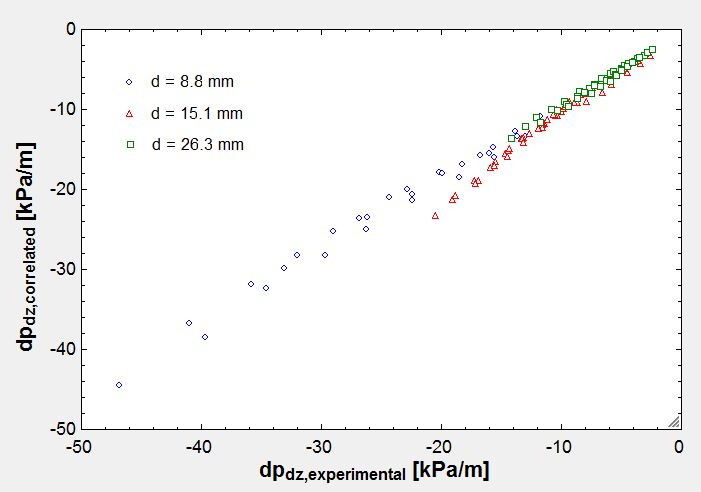
\includegraphics[width=10cm]{Part3_corr_v_exp_lo.jpg}\\

Figure 3.2 below plots the experimental vapor mass flow rate and diameter values against the correlated pressure gradient values from the optimized correlation of case 1. The lines/curves that formed for each given diameter are a result of different liquid flow rate values. Regardless, this graph confirms a trend that the pressure gradient decreases as the vapor flow rate increases, but, more importantly, the rate at which the pressure gradient decreases increases with increasing pipe diameter.

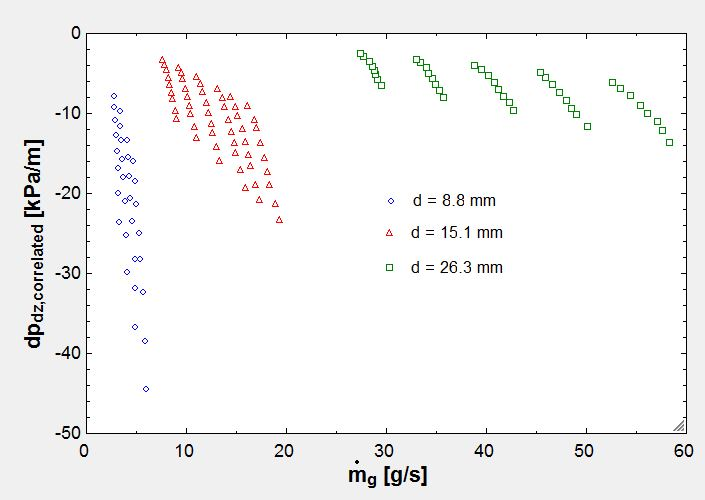
\includegraphics[width=10cm]{Part3_m_dot_lo.jpg}\\

\textbf{Discussion}

The strategy used to estimate these \(C\)-values values is not perfect, and was selected to comply with time constraints. As demonstrated in miscellaneous trail runs, initially iterating calculations over every combination of \(C_1\) and \(C_2\) between \(-1\) and \(1\) with steps of \(0.001\) might have yielded much different but more accurate \(C\)-values to three decimal places. Extending the \((-1,1)\) range of the \(C\)-values might have done the same. However, running so many iterations takes much longer and yields what seems to be only small improvements in MAE values. If time allowed, iterations would be run over a much larger range of \(C\)-values to acquire more optimal results. 


\end{document}
